% Copyright 2013 Nicolai Hähnle <nhaehnle@gmail.com>
%
% This work is licensed under the Creative Commons Attribution-ShareAlike 3.0
% Unported License, see http://creativecommons.org/licenses/by-sa/3.0/
%
% Among other things, this means that yes, you may take e.g. illustrations from
% the book and use them in your own work. However, (a) you must give proper
% attribution by naming me as its original author and (b) you must make your
% derivative work available under the same or similar license terms.
%
% See the Creative Commons website for the exact licensing terms.

\chapter{The Voronoi Cell of a Lattice and its Applications}
\label{chapter:voronoi-cell}

The Voronoi diagram of a point set is defined
to provide the answer to the closest vector problem:
given a point set $P$,
the Voronoi cell of $x \in P$ is the set of points
that are closer to $x$ than to any other point in $P$.

In this chapter, we will see how the Voronoi diagram of a lattice
can be used to solve both the shortest and the closest vector problem
in single exponential time by a deterministic algorithm.
Considering how early Voronoi diagrams were first studied,
and how obvious their usefulness seems in hindsight,
it took a very long to find this algorithm
which is due to Micciancio and Voulgaris~\cite{MR2743283}.


\section{The Voronoi cell of a lattice}

\begin{definition}
  Let $\Lambda \subset \R^d$ be a lattice.
  Let $x \in \Lambda \setminus \{ 0 \}$.
  We define the open half-space
  \[
    H_x := \{ p \in \R^d ~:~ \|p\|_2 < \|x-p\|_2 \}
  \]
  and the (open) \emph{Voronoi cell} of $\Lambda$
  \[
    \cV_\Lambda := \bigcap_{x \in \Lambda\setminus\{0\}} H_x
  \]
  Figure~\ref{fig:voronoi-diagram} shows a $2$-dimensional example.
\end{definition}

\begin{figure}
  \begin{center}
    \begin{tikzpicture}
      \clip (-2.2,-2.3) rectangle (2.2,4.3);

      \fill[black!10]
        (0,1.0625) -- (0.5,0.9375) -- (0.5,-0.9375) -- (0,-1.0625) --
        (-0.5,-0.9375) -- (-0.5,0.9375) --cycle;

      \foreach \y in {-1,0,1,2}
        \foreach \x in {-3,-2,-1,0,1,2}
          \fill ($\x*(1,0) + \y*(0.5,2)$) circle[radius=2pt];

      \draw (0,0) node[below] {$0$};

      \foreach \y in {-1,0,1,2}
        \foreach \x in {-4,-3,-2,-1,0,1,2}
          \draw ($\x*(1,0) + \y*(0.5,2)$) +(0,1.0625) -- +(0.5,0.9375) -- +(0.5,-0.9375) -- +(0,-1.0625);
    \end{tikzpicture}
  \end{center}
  \caption{The Voronoi diagram of a lattice. The Voronoi cell of $0$ is shaded.}
  \label{fig:voronoi-diagram}
\end{figure}

\begin{lemma}
  If $\Lambda$ is full-dimensional, $\overline{\cV_\Lambda}$ is a polytope.

  For a general lattice $\Lambda$,
  $\overline{\cV_\Lambda} = P + \langle \Lambda \rangle^\bot$
  where $P = \overline{\cV_\Lambda} \cap \langle \Lambda \rangle$ is a polytope.
\end{lemma}
\begin{proof}
  For linearly independent vectors $x_1, \ldots, x_d \in \Lambda$,
  we have
  \[
    \cV_\Lambda \subseteq
      \underbrace{H_{x_1} \cap \dots \cap H_{x_d} \cap H_{-x_1} \cap \dots \cap H_{-x_d}}_{=: Q}.
  \]
  The right hand side $Q$ is an open parallelepiped.
  In particular, it is bounded, so $\cV_\Lambda$ is bounded.

  Let $R > 0$ such that $Q \subseteq B(0,R)$.
  Every facet of $\overline{Q}$ lies on a hyperplane of the form
  \[
    \|p\|_2 = \|x - p\|_2 \iff 2p^Tx = x^Tx
  \]
  for some $x = \pm x_j$.
  Note that $\|p\|_2 \geq \frac{1}{2} \|x\|_2$ for all points $p$ on the facet.
  On the other hand, $\|p\|_2 \leq R$ by definition of $R$,
  so that we get $\|\pm x_j\|_2 \leq 2R$ for all $j$.

  We claim that
  \[
    \cV_\Lambda = \bigcap_{x \in \Lambda\setminus\{0\} ~:~ \|x\|_2 \leq 2R} H_x
  \]
  follows.
  The inclusion from left to right is clear from the definition.
  For the inclusion from right to left,
  let $p \in H_x$ for all $x \in \Lambda\setminus\{0\}$ with $\|x\|_2 \leq 2R$.
  In particular, this implies $p \in \overline{Q}$ and therefore $\|p\|_2 \leq R$.
  This in turn implies $p \in H_y$ for all $y$ with $\|y\|_2 > 2R$.
  To summarize,
  \[
     p \in \left( \bigcap_{x \in \Lambda\setminus\{0\} ~:~ \|x\|_2 \leq 2R} H_x \right)
      \cap \left( \bigcap_{y \in \Lambda\setminus\{0\} ~:~ \|y\|_2 > 2R} H_y \right) = \cV_\Lambda
  \]
  which implies the claim.
  That is, $\overline{\cV_\Lambda}$ is bounded and defined as the intersection of finitely many half-spaces,
  i.e., it is a polytope.

  The statement of the Lemma for general lattices follows
  directly from the observation that $x \in \Lambda$ is a closest lattice vector to $p$
  if and only if it is a closest lattice vector of the orthogonal projection $p'$ of $p$
  onto $\langle \Lambda \rangle$.
\end{proof}

Now that we have established that $\overline{\cV_\Lambda}$ is a polytope,
a natural algorithmic representation suggests itself:

\begin{definition}
  We say that $x \in \Lambda$ is \emph{Voronoi relevant} if
  \[
    \| p \|_2 \leq \| x - p \|_2 \iff 2p^Tx \leq x^T x
  \]
  is a facet-defining inequality of $\overline{\cV_\Lambda}$.
\end{definition}

Given a representation of $\cV_\Lambda$ in terms of Voronoi relevant vectors,
simple tasks such as testing whether a point is contained in $\cV_\Lambda$
can be solved in time $N \cdot \poly(d, b)$
where $b$ is the encoding size of the coordinates
and $N$ is the number of Voronoi relevant vectors.
Our first goal in this chapter will be to bound this number $N$.
Before we can do this -- and simultaneously show how those vectors
can be found -- we need some basic tools.

\begin{lemma}
  \label{lemma:voronoi-diagram-symmetry}
  Let $x \in \frac{1}{2} \Lambda$.
  The Voronoi diagram of $\Lambda$ is symmetric with respect to $x$.
\end{lemma}
\begin{proof}
  Since the symmetry $x + u \mapsto x - u$ preserves distances,
  we only need to show that the lattice $\Lambda$ is symmetric with respect to $x$.
  Whenever $x + u \in \Lambda$, we have
  \[
    x - u = (x + u) - 2u,
  \]
  where $u \in \frac{1}{2} \Lambda$.
  That is, $x - u \in \Lambda$ as well, completing the proof.
\end{proof}

\begin{lemma}
  \label{lemma:voronoi-relevant-facet-interior}
  Let $x \in \Lambda$ be a Voronoi relevant vector.
  Then $x/2$ lies in the relative interior of the associated facet of $\cV_\Lambda$.
\end{lemma}
\begin{proof}
  The facet associated to $x$ is
  \[
    F = \cV_\Lambda \cap \{ 2p^Tx = x^Tx \}
  \]
  The point $x/2$ lies on the hyperplane defining $F$,
  and by Lemma~\ref{lemma:voronoi-diagram-symmetry},
  the entire Voronoi diagram is symmetric with respect to $x/2$.
  In particular, $F$ is symmetric with respect to $x/2$.
  Since $F$ is convex, this implies the claim.
\end{proof}

\begin{lemma}
  \label{lemma:voronoi-relevant-as-closest}
  Let $x \in \Lambda$.
  Then $x$ is Voronoi relevant if and only if
  $0$ and $x$ are the unique closest lattice vectors to $\frac{1}{2} x$.
\end{lemma}
\begin{proof}
  Let $x$ be Voronoi relevant and
  assume that there is a third vector $y \in \Lambda$ that is equally close or closer.
  \begin{center}
    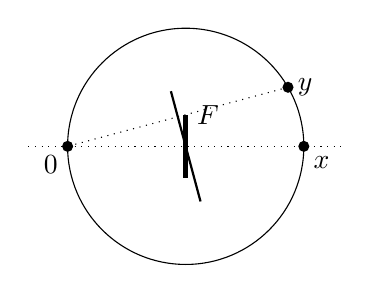
\begin{tikzpicture}
      \fill (0,0) circle[radius=2pt] node[below left] {$0$};
      \fill (3,0) circle[radius=2pt] node[below right] {$x$};
      \draw[dotted] (-0.5,0) -- (3.5,0);
      \draw[ultra thick] (1.5,-0.4) -- (1.5,0.4) node[right] {$F$};
      \draw (1.5,0) circle[radius=1.5cm];

      \fill (1.5,0) +(30:1.5) circle[radius=2pt] node[right] {$y$};
      \draw[thick] (1.5,0) +(0.188,-0.7) -- +(-0.188,0.7);
      \draw[dotted] (2.8,0.75) -- (0,0);
    \end{tikzpicture}
  \end{center}
  In this case, $x/2$ either lies on the hyperplane bounding $H_y$
  or is cut off by that hyperplane entirely.
  In any case, we have a contradiction with Lemma~\ref{lemma:voronoi-relevant-facet-interior}.

  Now suppose $0$ and $x$ are the unique closest lattice vectors to $\frac{1}{2} x$.
  By compactness, there is a neighborhood of $\frac{1}{2} x$
  in the bounding hyperplane $\partial H_x$
  for which $0$ and $x$ are the unique closest vectors as well.
  The neighborhood is therefore contained in $\overline{\cV_\Lambda}$,
  which means that there is a facet of $\overline{\cV_\Lambda}$ in $\partial H_x$,
  i.e., $x$ is Voronoi relevant.
\end{proof}



\section{Computing Voronoi relevant vectors}

A different perspective on the statement of Lemma~\ref{lemma:voronoi-relevant-as-closest}
is the following.
The point $x/2$ lies in the refined lattice $\frac{1}{2} \Lambda$,
to which we can associate a natural \emph{parity function},
see Figure~\ref{fig:lattice-refinement-parity} for an illustration:
\begin{align*}
  \sigma : \frac{1}{2} \Lambda &\to G := (\frac{1}{2} \Lambda) / \Lambda \cong (\Z_2)^d \\
                   u &\mapsto u + \Lambda
\end{align*}%
\begin{figure}
  \begin{center}
  \begin{tikzpicture}
    \clip (-1,-1) rectangle (4,3);
    \foreach \p/\color in {{(0,0)}/black,{(0.75,0.15)}/red,{(-0.05,0.85)}/green,{(0.7,1)}/blue}
      \foreach \x in {-1,0,1,2}
        \foreach \y in {-2,-1,0,1,2}
          \path[fill=\color] ($\x*(1.5,0.3) + \y*(-0.1,1.7)$) +\p circle[radius=2pt];
  \end{tikzpicture}
  \end{center}
  \caption{A lattice $\Lambda$ in black and its refinement $\frac{1}{2} \Lambda$
    with parities indicated using different colors.}
  \label{fig:lattice-refinement-parity}
\end{figure}%
The Lemma then says that for every Voronoi relevant vector $x \in \Lambda$,
there is a vector $u \in \frac{1}{2} \Lambda$ of non-zero parity
such that $0$ and $x$ are the unique closest vectors to $u$ in $\Lambda$.
For all vectors $u' \in \frac{1}{2} \Lambda$ with the \emph{same} parity $\sigma(u') = \sigma(u)$,
the relative location of closest vectors in $\Lambda$ is the same.
This suggests the following algorithm for finding Voronoi relevant vectors:
\begin{codebox}
  \Procname{$\proc{VoronoiCell}(\Lambda)$}
  \li $X \gets \emptyset$
  \li \For $U \gets \left((\frac{1}{2} \Lambda) / \Lambda\right) \setminus \{ 0 \}$
  \li \Do $u \gets$ representative of $U$
  \li     $x \gets \proc{CVP}(\Lambda, u)$
  \li     $X \gets X \cup \{ 2(x - u), 2(u - x) \}$
      \End
  \li \Return $X$
\end{codebox}
We are purposefully imprecise about how the lattice $\Lambda$ is represented
and how the closest vector problem is to be solved.
For now, the key point is that we can find all Voronoi relevant vectors
by solving $2^d - 1$ closest vector problems:

\begin{lemma}
  \label{lemma:voronoi-cell-computation}
  The set $X$ returned by \proc{VoronoiCell} contains all Voronoi relevant vectors.
\end{lemma}
\begin{proof}
  Let $y \in \Lambda$ be a Voronoi relevant vector.
  By Lemma~\ref{lemma:voronoi-relevant-as-closest},
  the vector $y/2 \in \frac{1}{2}\Lambda \setminus \Lambda$ has exactly two closest vectors,
  $0$ and $y$.

  There is one iteration of $\proc{VoronoiCell}$ in which $\sigma(u) = \sigma(y/2)$
  or, equivalently, $u \equiv y/2 \pmod{\Lambda}$.
  In this iteration, the closest vector subroutine must return
  either $x = u - y/2$ or $x = u + y/2$, see Figure~\ref{fig:voronoi-cell-computation}.
  In both cases, the algorithm adds $y$ and $-y$ to the set $X$.
\end{proof}
\begin{figure}
  \begin{center}
  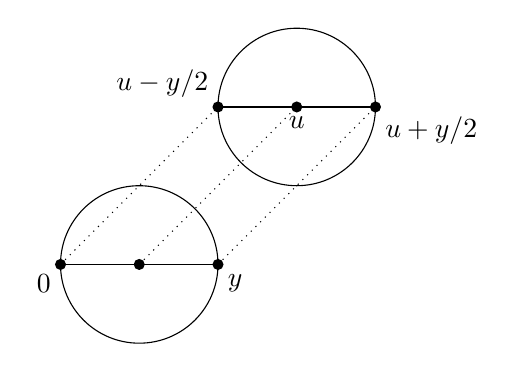
\begin{tikzpicture}
    \fill (0,0) circle[radius=2pt] node[below left] {$0$};
    \fill (2,0) circle[radius=2pt] node[below right] {$y$};
    \fill (1,0) circle[radius=2pt];
    \draw (1,0) circle[radius=1cm];
    \draw (0,0) -- (2,0);

    \fill (3,2) circle[radius=2pt] node[below] {$u$};
    \fill (4,2) circle[radius=2pt] node[below right] {$u + y/2$};
    \fill (2,2) circle[radius=2pt] node[above left] {$u - y/2$};
    \draw (3,2) circle[radius=1cm];
    \draw (2,2) -- (4,2);

    \draw[dotted] (0,0) -- (2,2);
    \draw[dotted] (1,0) -- (3,2);
    \draw[dotted] (2,0) -- (4,2);
  \end{tikzpicture}
  \end{center}
  \caption{Since $u \equiv y/2 \pmod\Lambda$, the set of closest vectors is identical after translation.}
  \label{fig:voronoi-cell-computation}
\end{figure}

\begin{example}
  The computed set $X$ may contain vectors that are not Voronoi relevant.
  Consider the case $\Lambda = \Z^2$ as shown below with its Voronoi cell.
  \begin{center}
    \begin{tikzpicture}
      \draw[fill=black!10] (-1,1) rectangle (1,-1) node[right] {$\overline{\cV_\Lambda}$};

      \foreach \x in {-1,0,1}
        \foreach \y in {-1,0,1}
          \fill ($\x*(2,0) + \y*(0,2)$) circle[radius=2pt];

      \draw (0,0) node[below] {$0$};

      \draw[fill=white] (1,1) circle[radius=2pt] node[right] {$u$};

      \draw (1,1) circle[radius=1.41cm];
    \end{tikzpicture}
  \end{center}
  During one iteration of the algorithm, $u$ will be as shown (or equivalent modulo $\Lambda$).
  There are four closest vectors to $u$, and no matter which of them is returned,
  the algorithm adds two vectors to $X$ that are not Voronoi relevant because
  the corresponding hyperplane $\partial H_x$ only induces
  a lower-dimensional face of $\overline{\cV_\Lambda}$.
\end{example}

If desired, we can detect vectors in $X$ that are not Voronoi relevant
using $O(N^2 d) = 2^{O(d)}$ arithmetic operations:
according to Lemma~\ref{lemma:voronoi-relevant-facet-interior},
it suffices to check every $x/2$ for $x \in X$ against every other $y \in X$
and compare distances.


\begin{corollary}
  \label{cor:number-of-voronoi-relevant}
  There are at most $2 \cdot (2^d - 1)$ Voronoi relevant vectors.
\end{corollary}



\section{Shortest and closest vectors via the Voronoi cell}

Now that we know how to compute the Voronoi cell,
let us see how it can be used.
First, we see that it contains a list of all shortest vectors of the lattice.

\begin{lemma}
  Let $x \in \Lambda$ be a shortest non-zero vector.
  Then $x$ is Voronoi relevant.
\end{lemma}
\begin{proof}
  Consider the ball of radius $\|x/2\|_2$ around $x/2$:
  \begin{center}
  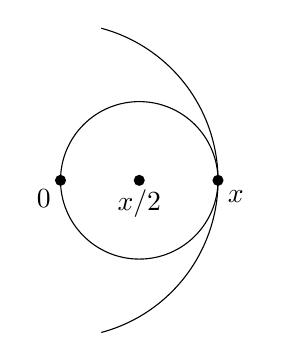
\begin{tikzpicture}
    \fill (0,0) circle[radius=2pt] node[below left]{$0$};
    \fill (2,0) circle[radius=2pt] node[below right]{$x$};
    \fill (1,0) circle[radius=2pt] node[below]{$x/2$};

    \draw (1,0) circle[radius=1cm];
    \draw (0,0) +(-75:2cm) arc[start angle=-75,end angle=75,radius=2cm];
  \end{tikzpicture}
  \end{center}
  Since $x$ is a shortest vector, $0$ and $x$ are the unique closest vectors to $x/2$.
  By Lemma~\ref{lemma:voronoi-relevant-as-closest}, $x$ is Voronoi relevant.
\end{proof}

\begin{corollary}
  Every lattice has at most $2 \cdot (2^d - 1)$ shortest vectors.
\end{corollary}

\begin{remark}
  Let us place spheres centered at every lattice point of a radius
  such that two spheres may touch but not overlap.
  The number of spheres that touch a fixed sphere is called the \emph{kissing number}
  of the sphere packing,
  and it is equal to the number of shortest vectors in the lattice.
  Hence, the previous Corollary is an upper bound on the kissing number
  of a lattice sphere packing.

  This bound happens to be tight for $d = 2$,
  but considerably better bounds are known in higher dimension.
  A classical source on the study of sphere packings is~\cite{MR1662447}.
\end{remark}

We can also use the Voronoi cell to compute closest vectors.
This may seem absurd at first,
because we needed to compute closest vectors in the first place to be able to
find the Voronoi relevant vectors.
However, if we need to solve \emph{many} closest vector problems,
then it may be useful to compute the Voronoi cell as a pre-processing step
to speed up future CVP computations.
We will apply this idea in Section~\ref{sec:voronoi-full-algorithm}.

For now, suppose we know the Voronoi cell $\cV$ of a lattice $\Lambda$
and are given a target vector $t \in \R^d$.
\begin{figure}
\begin{center}
  \begin{tikzpicture}
    \clip (-2.2,-2.3) rectangle (2.2,4.3);

    \foreach \y in {-1,0,1,2}
      \foreach \x in {-3,-2,-1,0,1,2}
        \fill ($\x*(1,0) + \y*(0.5,2)$) circle[radius=2pt];

    \draw (0,0) node[below] {$0$};

    \foreach \y in {-1,0,1,2}
      \foreach \x in {-4,-3,-2,-1,0,1,2}
        \draw ($\x*(1,0) + \y*(0.5,2)$) +(0,1.0625) -- +(0.5,0.9375) -- +(0.5,-0.9375) -- +(0,-1.0625);

    \coordinate (t) at (-1.1,3.7);
    \fill (t) circle[radius=2pt] node[left] {$t$};
    \draw (0,0) -- (t);
  \end{tikzpicture}
\end{center}
\caption{We find the Voronoi cell containing $t$ by tracing along the segment $[0,t]$.}
\label{fig:cvp-via-voronoi-cell-tracing}
\end{figure}
The problem of finding a closest lattice vector to $t$
is essentially the problem of finding the Voronoi cell translate that contains $t$.
We will solve that problem by following the line segment $[0,t]$,
see Figure~\ref{fig:cvp-via-voronoi-cell-tracing}.
\begin{codebox}
  \Procname{$\proc{CVP-via-Voronoi-Simple}(\Lambda, \cV_\Lambda, t)$}
  \zi $\cV_\Lambda$ is given by a list that contains all Voronoi relevant vectors
  \li $x \gets 0$
  \li \While $t \not\in x + \overline{\cV_\Lambda}$
  \li \Do Find the point $p$ where $[0,t]$ leaves $x + \cV_\Lambda$
  \li     Let $x' + \cV_\Lambda$, $x' \in \Lambda$, be the Voronoi cell entered at $p$
  \li     $x \gets x'$
      \End
  \li \Return $x$
\end{codebox}
Clearly, the algorithm returns a correct result when it terminates.
Each of the individual steps in this algorithm can be implemented in time $O(N \cdot \poly(d,b))$,
where $N$ is the size of the given list containing the Voronoi relevant vectors.
The test whether $t \in x + \overline{\cV_\Lambda}$ can be done by evaluating the $N$ linear functions
associated with the facets of $\overline{\cV_\Lambda}$.
Similarly, the point $p$ and the facet it lies on can be found by intersecting the line through $0$ and $t$
with each of the hyperplanes defining the facets of $x + \overline{\cV_\Lambda}$.

There is a subtle degenerate situation when the segment $[0,t]$ intersects a lower-dimensional
face of a cell $x + \overline{\cV_\Lambda}$.
This degeneracy can be avoided by an appropriate perturbation of the target vector $t$.

For now, let us simply assume that this degenerate situation does not happen
and continue bounding the running time of the algorithm.
Since the Voronoi cells are convex, every cell is entered at most once.
Since we only enter cells that intersect the segment $[0,t]$,
it suffices to bound the number of such cells
to bound the overall running time of the algorithm.

For every $x + \cV_\Lambda$ encountered in the algorithm,
we have $x \in [0,t] + \cV_\Lambda$
and therefore
\[
  x + \cV_\Lambda \subseteq [0,t] + 2 \cV_\Lambda
\]
Since the open cells are disjoint,
it suffices to bound the volume of $[0,t] + 2 \cV_\Lambda$.
\begin{lemma}
  Let $\lambda \in \R$ such that $t \in \lambda \cV_\Lambda$.
  Then \proc{CVP-via-Voronoi-Simple} visits at most $(\lambda+2)^d$ Voronoi cells of the lattice.
\end{lemma}
\begin{proof}
  By convexity, we have $[0,t] \subseteq \lambda \cV_\Lambda$,
  so that
  \[
    x + \cV_\Lambda \subseteq (\lambda + 2) \cV_\Lambda
  \]
  for every Voronoi cell visited by the algorithm.
  Hence, the number of such cells is bounded by
  \[
    \frac{\vol((\lambda + 2) \cV_\Lambda)}{\vol(x + \cV_\Lambda)}
      = \frac{(\lambda + 2)^d \vol \cV_\Lambda }{\vol \cV_\Lambda}
      = (\lambda + 2)^d \qedhere
  \]
\end{proof}
This seems to be a rather crude bound.
Intuitively, we expect a bound that is linear in the norm of $t$ for very large $t$.
But note that even such a bound -- and it is clear that we cannot possibly do better --
is exponential in the encoding size of $t$, which leads to an unacceptable running time.
The solution lies in geometric scaling, using two simple observations.
\begin{corollary}
  If $t \in 2\cV_\Lambda$,
  \proc{CVP-via-Voronoi-Simple} can be used to solve CVP in time $2^{O(d)} \poly(b)$.
\end{corollary}

The second observation is that the Voronoi cell of $k \Lambda$ is simply $k \cV_\Lambda$.
This means that if $t \not\in 2\cV_\Lambda$,
we can instead search for a closest vector $x'$ to $t$
in a sparser lattice $2^\kappa \cdot \Lambda$
that satisfies $t \in 2 \cdot 2^\kappa \cV_\Lambda$.
Once such a vector $x' \in \Lambda$ is found,
we can shift the problem by $-x'$,
thereby moving $t$ closer to the origin.
This is illustrated in Figure~\ref{fig:cvp-via-scaling}.

\begin{codebox}
  \Procname{$\proc{CVP-via-Voronoi-Scaling}(\Lambda, \cV_\Lambda, t)$}
  \li \If $t \in \cV_\Lambda$
  \li \Then \Return $0$
      \End
  \li $x' \gets \proc{CVP-via-Voronoi-Scaling}(2\Lambda, 2\cV_\Lambda, t)$
  \li $x'' \gets \proc{CVP-via-Voronoi-Simple}(\Lambda, \cV_\Lambda, t - x')$
  \li \Return $x' + x''$
\end{codebox}
Let $\kappa \in \N_0$ be minimal with $t \in 2^\kappa \cV_\Lambda$.
Then it is easy to see by induction over $\kappa$
that the recursion depth given input $t$ is exactly $\kappa$.

We see the correctness of the algorithm via induction over $\kappa$ as well.
It is self-evident if $\kappa = 0$, i.e., $t \in \cV_\Lambda$.
Suppose $\kappa \in \N_0$ is minimal with $t \in \cV_\Lambda$ and $\kappa \geq 1$.
Then we find, by the induction hypothesis,
$x' \in 2\Lambda$ such that $t \in x' + 2\cV_\Lambda$.
We also find $x'' \in \Lambda$ with $(t-x') \in x'' + \cV_\Lambda$,
and therefore $t \in (x' + x'') + \cV_\Lambda$,
which means the returned lattice vector is a closest vector to $t$.

Since we have $(t - x') \in 2\cV_\Lambda$,
each call of $\proc{CVP-via-Voronoi-Simple}$
takes time $2^{O(d)} \poly(b)$.
That is, the overall running of the algorithm is essentially $\kappa \cdot 2^{O(d)} \poly(b)$.
The recursion depth $\kappa$ is bounded by $\log \|t\|_2$ if $\Lambda \subseteq \Z^d$.
That is, after an appropriate scaling, we get:

\begin{theorem}
  Given a list of Voronoi relevant vectors,
  $\proc{CVP-via-Voronoi-Scaling}$ computes a closest vector to $t$ in time $2^{O(d)} \poly(b)$.
\end{theorem}


\begin{figure}
\begin{center}
  \begin{tikzpicture}
    \clip (-2.2,-2.3) rectangle (2.2,4.3);

    \foreach \y in {-1,0,1,2}
      \foreach \x in {-3,-2,-1,0,1,2}
        \fill[black!40] ($\x*(1,0) + \y*(0.5,2)$) circle[radius=2pt];

    \draw (0,0) node[below] {$0$};

    \foreach \y in {-1,0,1,2}
      \foreach \x in {-4,-3,-2,-1,0,1,2}
        \draw[black!40] ($\x*(1,0) + \y*(0.5,2)$) +(0,1.0625) -- +(0.5,0.9375) -- +(0.5,-0.9375) -- +(0,-1.0625);

    \coordinate (t) at (-1.1,3.7);
    \fill (t) circle[radius=2pt] node[left] {$t$};
    \draw (0,0) -- (t);
    \draw (-1,4) node[right] {$x'$};

    \foreach \y in {0,2}
      \foreach \x in {-2,0,2}
        \fill ($\x*(1,0) + \y*(0.5,2)$) circle[radius=2pt];

    \foreach \y in {-2,0,2}
      \foreach \x in {-4,-2,0,2}
        \draw ($\x*(1,0) + \y*(0.5,2)$) +(0,2.125) -- +(1.0,1.875) -- +(1.0,-1.875) -- +(0,-2.125);

  \end{tikzpicture}
\end{center}
  \caption{Solving the closest vector problem via \proc{CVP-via-Voronoi-Scaling}.}
  \label{fig:cvp-via-scaling}
\end{figure}



\section{A single exponential time algorithm for computing the Voronoi cell}
\label{sec:voronoi-full-algorithm}

We find ourselves in an oddly circular situation.
Given some way of computing closest vectors in $\Lambda$,
we can also compute its Voronoi relevant vectors,
and given a way of computing its Voronoi relevant vectors,
we can also compute closest vectors in $\Lambda$.
\begin{center}
  \begin{tikzpicture}
    \node[left,inner sep=3mm,draw] (cvp) at (0,0) {Closest vectors};
    \node[right,inner sep=3mm,draw] (vc) at (3,0) {Voronoi cell};

    \draw[->] ($(cvp.east) + (0,-0.1)$) -- ($(vc.west) + (0,-0.1)$);
    \draw[->] ($(vc.west) + (0,0.1)$) -- ($(cvp.east) + (0,0.1)$);
  \end{tikzpicture}
\end{center}
We will break out of this cycle by a strengthening of the nearest plane method
of Section~\ref{sec:nearest-plane-approximation}.
Given an LLL-reduced basis $B$ of $\Lambda$,
we will see how a closest vector problem in $\Lambda$
can be solved by $2^{d/2}$ closest vector problems in $\Lambda' = \Lambda(b_1,\ldots,b_{d-1})$.

Each of those closest vector problems can be solved using the Voronoi cell of $\Lambda'$,
which has to be computed only once.
The circular dependency above becomes a linear chain of dependencies
in which we compute Voronoi cells of lattices of successively higher dimension,
see Figure~\ref{fig:voronoi-cell-dimension-reduction}.

The key point of the construction is that
even though up to $2^{O(d)}$ closest vector problems are solved in each dimension,
only one Voronoi cell needs to be computed in each dimension.
Hence the overall running time remains singly exponential.
\begin{figure}
  \begin{center}
    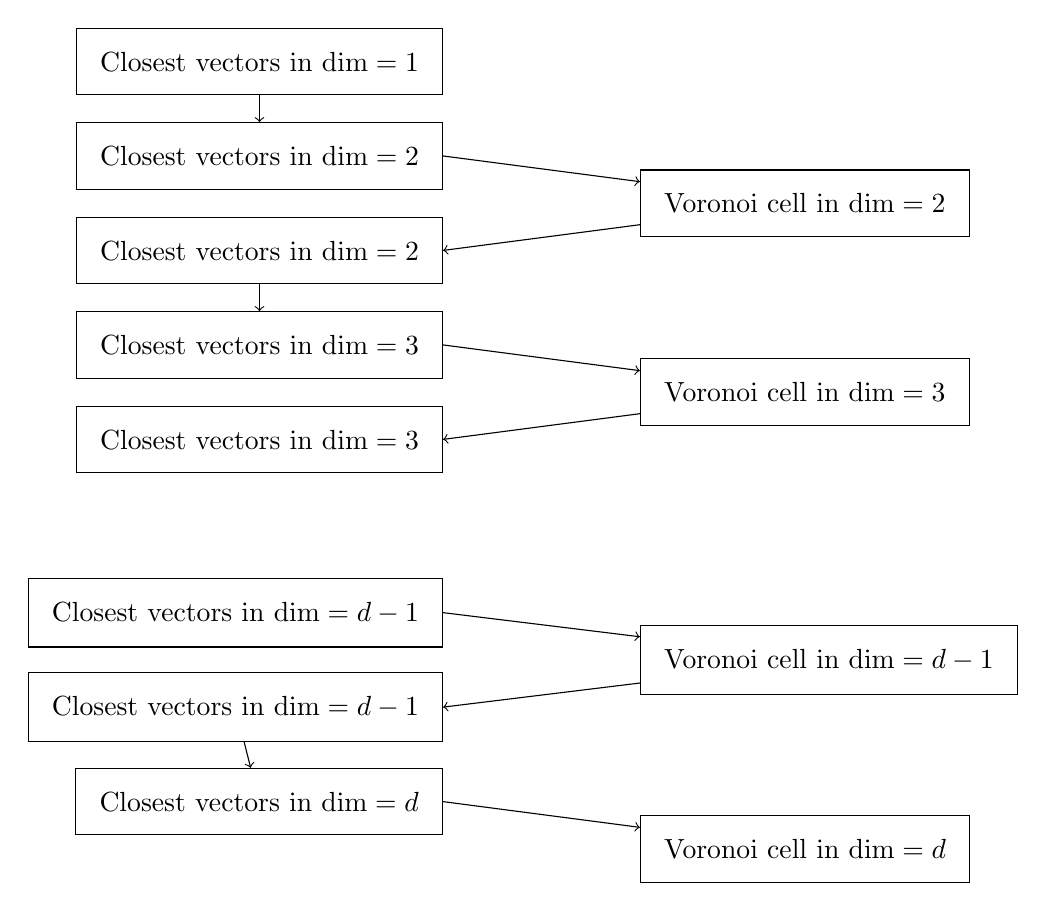
\begin{tikzpicture}
      \node[left,inner sep=3mm,draw] (cvp1) at (0,0) {Closest vectors in $\dim = 1$};
      \node[left,inner sep=3mm,draw] (cvp2a) at (0,-1.2) {Closest vectors in $\dim = 2$};
      \node[right,inner sep=3mm,draw] (vc2) at (2.5,-1.8) {Voronoi cell in $\dim = 2$};
      \node[left,inner sep=3mm,draw] (cvp2b) at (0,-2.4) {Closest vectors in $\dim = 2$};
      \node[left,inner sep=3mm,draw] (cvp3a) at (0,-3.6) {Closest vectors in $\dim = 3$};
      \node[right,inner sep=3mm,draw] (vc3) at (2.5,-4.2) {Voronoi cell in $\dim = 3$};
      \node[left,inner sep=3mm,draw] (cvp3b) at (0,-4.8) {Closest vectors in $\dim = 3$};

      \node[left,inner sep=3mm,draw] (cvpca) at (0,-7.0) {Closest vectors in $\dim = d-1$};
      \node[right,inner sep=3mm,draw] (vcc) at (2.5,-7.6) {Voronoi cell in $\dim = d-1$};
      \node[left,inner sep=3mm,draw] (cvpcb) at (0,-8.2) {Closest vectors in $\dim = d-1$};
      \node[left,inner sep=3mm,draw] (cvpda) at (0,-9.4) {Closest vectors in $\dim = d$};
      \node[right,inner sep=3mm,draw] (vcd) at (2.5,-10.0) {Voronoi cell in $\dim = d$};

      \draw[->] (cvp1) -- (cvp2a);
      \draw[->] (cvp2a.east) -- (vc2);
      \draw[->] (vc2) -- (cvp2b.east);
      \draw[->] (cvp2b) -- (cvp3a);
      \draw[->] (cvp3a.east) -- (vc3);
      \draw[->] (vc3) -- (cvp3b.east);

      \draw[->] (cvpca.east) -- (vcc);
      \draw[->] (vcc) -- (cvpcb.east);
      \draw[->] (cvpcb) -- (cvpda);
      \draw[->] (cvpda.east) -- (vcd);
    \end{tikzpicture}
  \end{center}
  \caption{Iteratively building Voronoi cells of larger dimension.}
  \label{fig:voronoi-cell-dimension-reduction}
\end{figure}

Let us recall the nearest plane method, see Figure~\ref{fig:nearest-plane-approximation}.
In Section~\ref{fig:nearest-plane-approximation},
we saw that if the basis $B$ is LLL-reduced,
there is a vector $x \in \Lambda$ such that
\[
  \|x-t\|_2^2 \leq 2^{d-2} \|b_d^\star\|_2^2
\]
Since $\|b_d^\star\|_2$ is the distance between adjacent lattice hyperplanes,
it follows that a closest vector to $t$ must lie,
if not on the nearest lattice hyperplane,
then on one of the $2 \cdot 2^{(d-2)/2} = 2^{d/2}$ lattice hyperplanes closest to $t$.
By projecting $t$ orthogonally onto each of those hyperplanes in turn
and solving a closest vector problem in $\Lambda'$,
we are guaranteed to find a closest vector.

\begin{theorem}
  The Voronoi relevant vectors of a lattice can be computed in time $2^{O(d)} \poly(b)$.
  As a consequence, the shortest and closest vector problems can be solved in the same asymptotic
  running time.
\end{theorem}






\section*{Exercises}

\begin{enumerate}
  \item
    \begin{enumerate}[(a)]
    \item Show that $(\frac{1}{2} \Lambda) / \Lambda \cong (\Z_2)^d$.

    \item Show that $|(\Z_2)^d| = 2^d = \frac{\det\Lambda}{\det \frac{1}{2} \Lambda}$.
    \end{enumerate}

  \item
    Define a suitable parity function on $\Lambda$ such that:
    \begin{enumerate}[(i)]
      \item A lattice vector of parity $0$ cannot define a facet of $\cV_\Lambda$.

      \item Given two vectors $x, y \in \Lambda$, $y \neq \pm x$, of the \emph{same} parity,
        show that at least one of them does not define a facet of $\cV_\Lambda$.
    \end{enumerate}
    Conclude with an alternative proof of the statement of Corollary~\ref{cor:number-of-voronoi-relevant}:
    there can be at most $2 \cdot (2^d - 1)$ Voronoi relevant vectors.
\end{enumerate}
